\chapter{Der Zerfall bei LHCb}
\label{chap:3}
%
\section{Der Large Hadron Collider}
%
Der \textit{Large Hadron Collider} (LHC) am CERN (Meyrin, Schweiz) ist der derzeit leistungsstärkste Teilchenbeschleuniger der Welt. Er dient der Erzeugung von Proton-Proton-Kollisionen ($pp$-Kollisionen) einer Schwerpunktenergie von bis zu $\sqrt{s}=\SI{14}{\tera\electronvolt}$\cite{lhc}. Diese Energien werden nach dem letzten Update mit $\SI{13}{\tera\electronvolt}$ beinahe ausgereizt\cite{lhc}. Durch die Ausweitung des zu untersuchenden Energiebereiches auf diese Größenordnung eignet sich der LHC zur Entdeckung von Physik jenseits des SM, wie etwa unbekannter Teilchen. Im Jahre 2012 gelang der ATLAS- und der CMS-Kollaboration die Entdeckung des in den 60er-Jahren von Higgs und Englert vorhergesagten Higgs-Bosons\cite{higgs}.
Bevor die Protonen im bis zu $\SI{90}{\meter}$ unter der Erde liegenden, $\SI{27}{\kilo\meter}$ langen Speicherring auf die maximale Schwerpunktsenergie beschleunigt werden, durchlaufen sie ein vielschrittiges System aus Vorbeschleunigern. Dessen letzte Stufe ist der \textit{Super Proton Synchrotron} (SPS), welcher die Protonen auf etwa $\SI{99,99978}{\percent}$ der Lichtgeschwindigkeit beschleunigt\cite{lhc}. Diese Protonen werden mit einer Schwerpunktsenergie von $\SI{0,45}{\tera\electronvolt}$ über zwei Transferlinien in den LHC injiziert, wo sie in entgegengesetzter Richtung beschleunigt werden. Die Beschleunigung und Kreisführung findet dabei in einem ultrahoch Vakuum über supraleitende Magnete, welche von flüssigem Helium auf etwa $\SI{1,9}{\kelvin}$ gekühlt werden, statt. So werden Hunderte einzelner Protonenbündel (\textit{bunches}) auf beinahe Lichtgeschwindigkeit beschleunigt und anschließend in Abständen von $\SI{25}{\nano\second}$ ($\SI{40}{\mega\hertz}$) in einem der vier großen Experimente durch Strahlkreuzung zur Kollision gebracht.
%
\section{Der LHCb Detektor}
%
\begin{figure}[H]
  \centering
      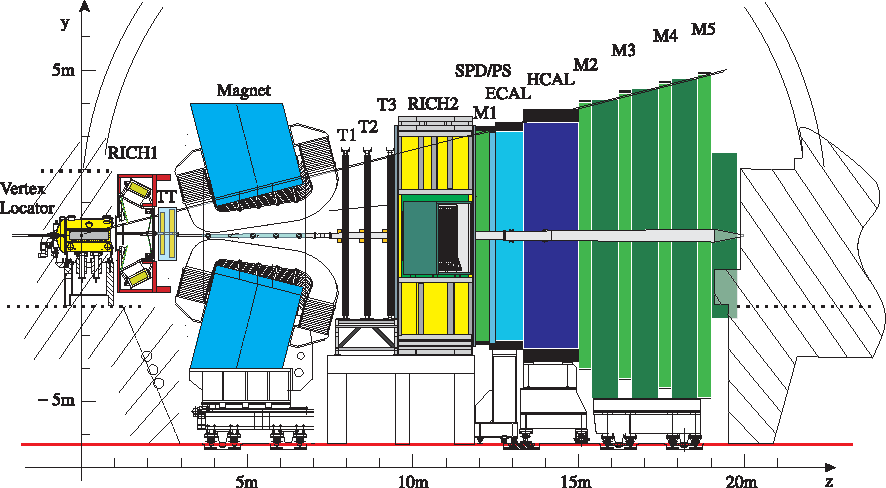
\includegraphics[width=\textwidth]{Plots/lhcb.pdf}
  \caption{Querschnitt des LHCb-Detektors.\cite{lhcb}}
  \label{fig:lhcb}
\end{figure}
%
Der LHCb Detektor deckt im Gegensatz zu den anderen drei Experimenten am LHC bei seinen Messungen nicht den gesamten Raumwinkel um den Kollisionspunkt ab. Es handelt sich hierbei um einen einarmigen vom Kollisionspunkt in Strahlrichtung vorwärtsgerichteten Detektor. Die Wahl dieser Bauart hängt unter anderem mit dem Hauptverwendungszweck des Detektors zusammen: wie der Name schon impliziert ist die Untersuchung von $b$-Quarks bzw. B-Mesonen Ziel des Experimentes. Da sich diese nach ihrer Erzeugung in den $pp$-Kollisionen in Kegeln unter sehr kleinen Winkeln zum Protonstrahl bewegen, ist ein Detektor wie der LHCb auf die Vermessung dieses Bereiches optimal ausgelegt, da einer der beiden Zerfallskegel genau in den Detektor strahlt. Der Akzeptanzbereich des Detektors zur Strahlachse gemessen beträgt hierbei $10$mrad - $300$mrad. Abbildung~\ref{fig:lhcb_angle} zeigt die Verteilung der $b$-Quarks auf den Raumwinkel, sowie in rot den Akzeptanzbereich von LHCb. Dieser deckt bei einer Schwerpunktsenergie von $\SI{8}{\tera\electronvolt}$ etwa $\SI{27}{\percent}$ der $b$-Quarks ab\cite{rad}.\\
%
\begin{figure}[H]
  \centering
      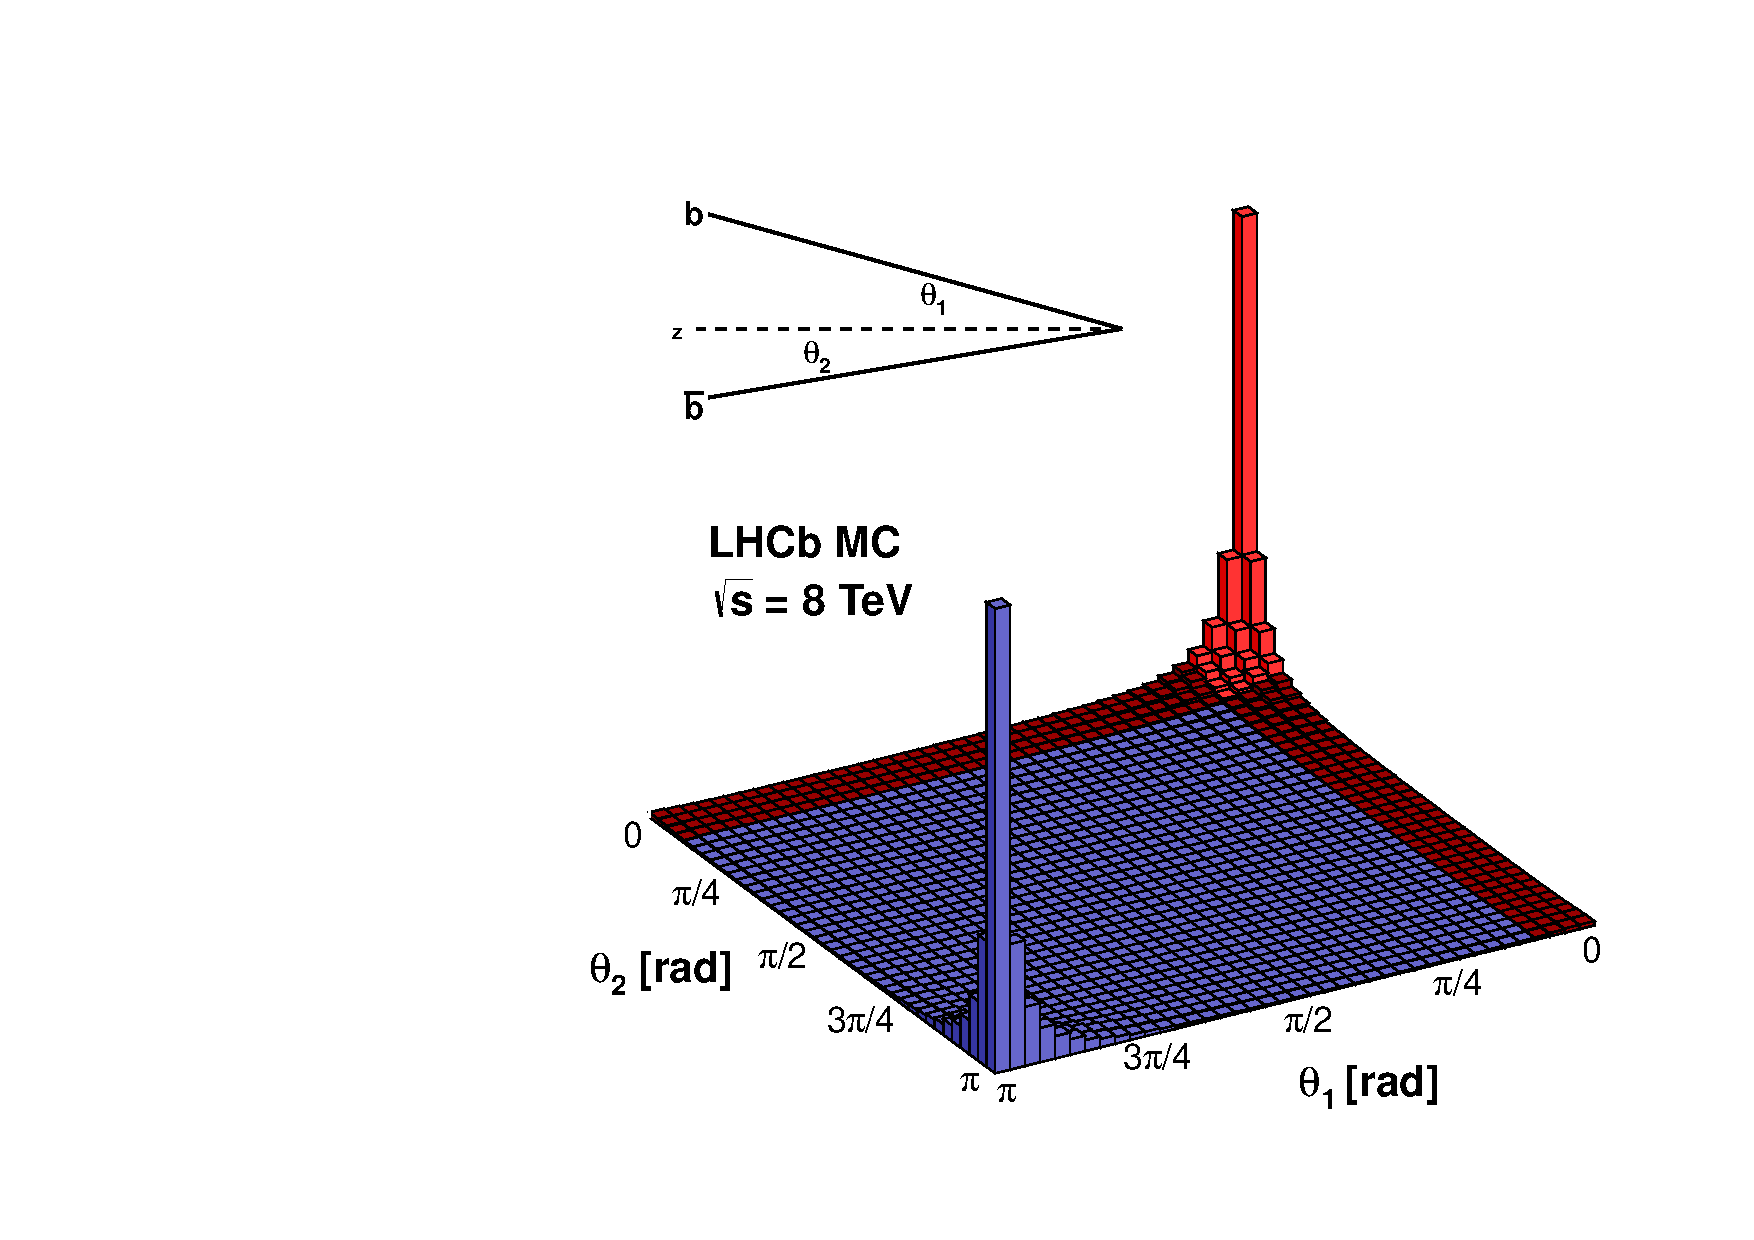
\includegraphics[width=0.8\textwidth]{Plots/08_rad_acc_scheme_left.pdf}
  \caption{Verteilung der $b$-Quarks auf den Raumwinkel, sowie in rot der Akzeptanzbereich von LHCb\cite{rad_pic}.}
  \label{fig:lhcb_angle}
\end{figure}
%
Der etwa $\SI{20}{\meter}$ lange Detektor ist aus mehreren Schichten verschiedener Detektoren und Messsysteme aufgebaut, die im Folgenden genauer erläutert werden. Dabei ist wenn von positiver z-Richtung die Rede ist, die Strahlrichtung vom Kollisionspunkt in den Detektor gemeint. Die Detektorsysteme lassen sich allgemein in zwei Arten von Detektoren unterteilen:
%
\begin{enumerate}
  \item Spurdetektoren: Vertex Locator (VELO), Trigger Tracker (TT), Innerer Tracker (IT), Äußerer Tracker (OT)
  \item Teilchenidentifikation (PID): erster und zweiter Cherenkovdetektor (RICH 1 und RICH 2), elektromagnetisches und hadronisches Kalorimeter (ECAL und HCAL) sowie die Myondetektoren.
\end{enumerate}
%
Der dem Kollisionspunkt am nächsten liegende Detektor ist der \textit{vertex locator}, kurz VELO. Seine Aufgabe ist die möglichst exakte Ermittlung der Zerfallsvertices der B-Mesonen. Die in den Kollisionen entstehenden B-Mesonen zerfallen innerhalb von Strecken einiger Millimeter, weswegen die Detektoren unmittelbar um den Kollisionspunkt liegen, wenn Daten genommen werden\cite{velo}. Da diese Region auch die am intensivsten von Strahlenschäden betroffene Region ist, ist der Detektor bei Bedarf mechanisch auf Abstand zu bringen.
%
\begin{figure}[H]
  \centering
      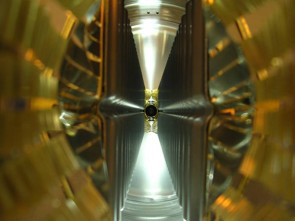
\includegraphics[width=0.6\textwidth]{Plots/VELO-beam-view.jpg}
  \caption{Ansicht des VELO-Detektors aus Strahlrichtung. Die halbmondförmigen Scheiben sind rechts und links vom Strahlengang angeordnet\cite{velo}.}
  \label{fig:velo}
\end{figure}
%
Wie in Abbildung~\ref{fig:velo} rechts und links erkennbar, umgibt der VELO den Strahlengang von zwei Seiten. Er besteht dabei im Einzelnen aus halbmondförmigen, $\SI{0.3}{\milli\meter}$ starken Scheiben von Spurdetektoren, die entlang des Strahlenganges angeordnet sind\cite{velo}. Die Messung der Zerfallspunkte findet dabei über die Bestimmung der $(r, \phi)$-Koordinaten innerhalb der Silikonsensoren statt. Dazu sind radial nach außen laufende Silikonstreifen ($\phi$) mit zirkular laufenden ($r$) kombiniert\cite{lhcb}. Durchqueren geladene Teilchen die Fasern, so erzeugen sie im Festkörper Elektron-Loch-Paare, welche eektronisch gemessen werden können und analog ausgelesen werden. Der während der Datennahme lediglich $\SI{7}{\milli\meter}$ vom \textit{beam} entfernte VELO stellt den Hauptspurdetektor vor Einsatz des Magneten dar\cite{velo}. \\
%
Dann Trigger Tracker.
